\chapter{Introducción}
\label{cap:intro}

\section{Antecedentes y motivación}
\label{intro:motivacion}

La gran contribución de información en la Internet se ha debido al origen de la Web 2.0, donde ésta se caracteriza por la participación activa del usuario, siendo reflejado en el auge de blogs, redes sociales u otras aplicaciones web \citep{web2007oberhelman}. Debido a lo anterior, se crean sistemas de procesamiento para grandes cantidades de información generadas por la interacción entre los usuarios.

Es así como con el tiempo se han ido creando distintas aplicaciones de \textsl{streaming}, debido al interesante funcionamiento que poseen, las que se caracterizan por ser capaces de procesar grandes flujos de datos en tiempo real \citep{ChenZ14a}. La necesidad de procesar informaci\'on en tiempo real surge dado que muchas aplicaciones, donde sus usuarios requieren de respuestas r\'apidas y actualizadas que le permitan tomar decisiones en per\'iodos cortos de tiempo. Dentro de los ejemplos existentes se encuentran; análisis de sentimientos de los mensajes de usuarios, análisis de los precios de la bolsa de valores, recopilación de información en caso de emergencia, entre otros. Las distintas aplicaciones que se han creado se volvieron críticas para sus usuarios, debido que sustenta la toma de decisiones de empresas o instituciones \citep{Wenzel14}.

Entre los sistemas actuales de procesamiento de \textsl{streaming} se encuentran S4 \citep{s4yahoo}, Storm \citep{stormtwitter}, Samza \citep{samza}, entre otros, los cuales son los más utilizados como arquitectura de procesamiento en la confección de distintas aplicaciones de \textsl{streaming}. Aunque poseen bastante flexibilidad para la creación de un sistema, por la facilidad de crear distintas topologías, no lo tiene para adaptarse en el tiempo, debido a que las topolog\'ias de procesamiento generadas son est\'aticas, por lo que dada la naturaleza din\'amica de las interacciones pueden surgir problemas de sobrecarga.

El problema de sobrecarga conlleva a una baja en el rendimiento, produciendo una pérdida de recursos, tiempo o información. Abortar este problema es cr\'itico, puesto que implica una mejora en la exactitud y disminución en el tiempo de procesamiento, debido que al tener mayor cantidad de datos, menor tiempo de procesamiento, se mejora la información entregada. Un ejemplo de esto, es que se posee un tiempo $t$ para procesar $n$ datos, de disminuir el tiempo de procesamiento total de los datos, se tendrá que en el mismo tiempo $t$ se procesarán una cantidad $n+m$ de datos, donde $m$ son los datos adicionales a analizar debido a la mejora del rendimiento. Como existe una mejora en la cantidad de datos para analizar, la información de salida es más exacta, debido que tiene más datos con que comparar. De esta manera, se efectúa una mejora en los recursos utilizados, debido a la disminución del tiempo de procesamiento, y una mejor calidad en la información entregada al usuario.

\section{Descripción del problema}
\label{intro:problema}

Entre los diferentes motores de procesamiento de datos masivos, existen los motores de \textsl{streaming}, los cuales reciben grandes cantidades de datos que deben procesar de forma distribuida y \textsl{online}. Para realizar esto, se requiere un cambio en el paradigma \textsl{bash processing}, el cual guarda los datos en una base de datos, los cuales luego son procesados de forma \textsl{offline} \citep{HawwashN14}, a uno que procese de forma \textsl{online}. Por lo que el paradigma cambia a uno basado en grafos, donde a través del cual fluye un \textsl{stream} de datos que es procesamiento por el conjunto de operadores que lo componen, los operadores corresponden a los nodos del grafo y las aristas a los flujos de datos preprocesados que salen del operador \citep{Shahrivari14}.

El modelo de procesamiento que se muestra en la Figura \ref{fig:grafo}, corresponde a un SPE (Sistema de Procesamiento de Eventos). Los vértices corresponden a operadores, como por ejemplo analizadores de sentimientos, filtros de palabras o algún algoritmo en particular, y las aristas corresponden a los flujos de datos entre un operador y otro. Además de esto, se tiene una fuente de datos, la cual entrega los datos iniciales a los primeros operadores del grafo \citep{AppelFFB12}.

\begin{figure}[ht!]
  \centering
    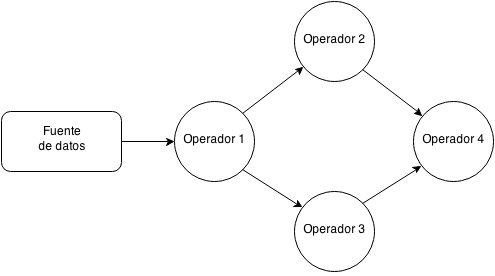
\includegraphics[scale=0.5]{images/Grafo.png}
  \caption{Ejemplo de modelo de SPE.}
  \label{fig:grafo}
\end{figure}

Cada motor de procesamiento de \textsl{streaming} está basado en un modelo de procesamiento en particular. Por ejemplo, S4 está basado en el modelo de procesamiento \textsl{push} \citep{s4yahoo}, y Storm en el modelo \textsl{pull} \citep{stormtwitter}. El primer modelo consiste en el envío de datos desde el operador. La ventaja de este modelo empleado por S4 radica en la abstracción en el envío de datos, sin embargo no asegura el procesamiento de estos, debido a que no existe un mensaje de respuesta al ser entregado al operador. En cambio, en el segundo modelo se basa en la petición de datos a un operador, por lo que son enviados solo si son requeridos. Si bien este modelo asegura procesamiento de los datos, genera una menor abstracción al programador, dado que en el primer modelo sólo se programa a que operador debe ir, en cambio en el segundo se debe indicar quién lo envía y quién lo recibe.

Pues bien, independiente del método que se utilice, existe un problema en la distribución, dado el dinamismo de los datos a procesar, pudiendo generarse sobrecargas en algún operador. Esto se produce dado que la tasa de procesamiento es menor a la tasa de llegada, generando colas en el sistema \citep{queueingtheory}. Por ejemplo, si se posee una tasa de llegada $\lambda$ y una tasa de servicio $\mu$, donde $\mu < \lambda$, se generan colas en el sistema, debido que se procesa más lento de lo que llegan los datos. Como existen colas, es necesario un aumento del rendimiento del sistema, debido que $\rho > 1 $, donde se define $\rho = \frac{\lambda}{s\mu}$, siendo $s$ la cantidad de servicios disponibles.

El caso más simple de modelo de SPE, existe una réplica por cada operador, de esta manera, cada servicio tendrá un valor de 1. Por lo tanto, al crear réplicas de cada uno de los servicios, se aumenta el rendimiento del sistema, en caso de haber colas. Para no utilizar recursos de forma excesiva, es necesario realizar el proceso de forma elástica, la cual se define como el aumento o disminución de la cantidad de servicios según la cantidad requerida por el sistema.

%Por lo tanto, es importante dar solución a las sobrecargas en los operadores, de tal manera que haya una menor tiempo promedio de espera en el procesamiento de los datos. Además, se tiene una mayor exactitud en los datos entregados, debido que la información entregada es más pŕoxima al tiempo real.

Es importante dar una solución al problema de sobrecarga de los operadores, para disminuir el tiempo del  procesamiento y aumentar la precisión de los resultados del sistema. Por lo tanto, dada la falta de flexibilidad del modelo de procesamiento de \textsl{streams}, surge un problema basado en la sobrecargada de los operadores más demandados. Esto debido a que no existe una forma de disminuir la sobrecarga y reducir las colas de espera, para mejorar el rendimiento del sistema y obtener información cercana al tiempo real.

\section{Solución propuesta}
\label{intro:solucion}

La solución propuesta consiste en el dise\~no de algoritmos de predicci\'on y distribuci\'on de carga a nivel de la l\'ogica del grafo. En la Figura \ref{fig:opt} se muestran los cuatro módulos que componen la estructura del m\'odelo propuesto para el dise\~no de los algoritmos, los cuales se componen por el monitor de carga, analizador de carga, predictor de carga y administrador de réplicas.

\begin{figure}[ht!]
  \centering
    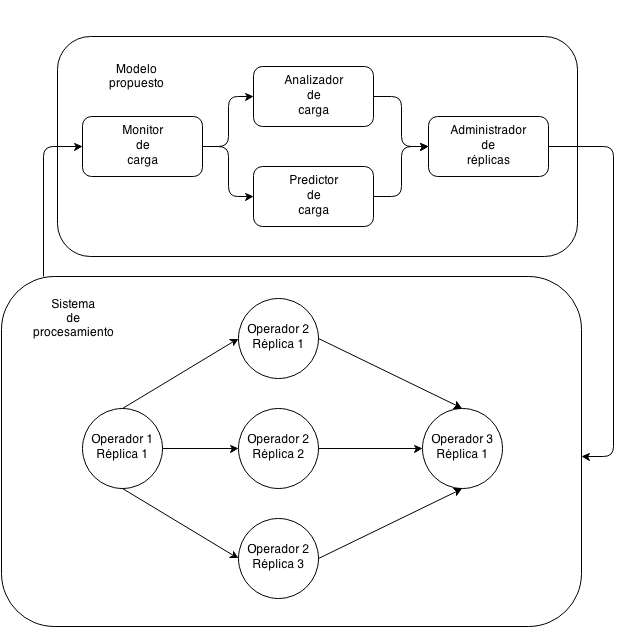
\includegraphics[scale=0.5]{images/Diagrama.png}
  \caption{Estructura del sistema de operadores y modelo propuesto.}
  \label{fig:opt}
\end{figure}

El monitor de carga está encargado de recuperar el nivel de carga de cada uno de los operadores. Esta información es entregada a otros dos módulos, los cuales están encargados de procesarla de tal manera de ver si existe alguna sobrecarga. Cada uno de éstos trabaja de forma independiente y tiene distintos métodos, uno proactivo y otro reactivo, de tal manera de poseer mayor exactitud en la detección de una sobrecarga.

El analizador de carga consiste en un método reactivo, el cual analiza el tráfico de los operadores en el tiempo actual, y cuantifica su carga. La sobrecarga de cada operador depende de un umbral, por lo que según ésto se envía al administrador de réplica el tráfico de cierto operador de ser necesario una replicación.

El predictor de carga consiste en un método proactivo, el cual analiza la carga de los distintos operadores según una ventana de tiempo, y predice la carga según un método predictivo. De esta manera, se determina la posible carga que existe en cierto período de tiempo futuro, donde según un umbral y un margen de error se envía el tráfico de carga de un operador al administrador de réplicas, y así analizar si es necesario una replicación.

El administrador de réplicas se alimenta de la información entregada por los dos módulos anteriores, y así toma una decisión de la administración de cada una de las réplicas de los distintos operadores. Por lo tanto, verifica cuántas réplicas son necesarias según la cantidad de tráfico de cierto operador.

Finalmente, el sistema de procesamiento constantemente está realizando un \textsl{feedback} al sistema de optimización, de tal manera que pueda administrar las réplicas necesarias.

%HIPOTESIS
Este sistema dar\'a un procesamiento más rápido de la información entregada en el sistema de procesamiento \textsl{online} de datos, a través de un proceso de optimización que posea bajo \textsl{overhead}.


\section{Objetivos y alcance del proyecto}
\label{intro:objetivos}

\subsection{Objetivo general}
	Dise\~no, construcción y evaluaci\'on de un algoritmo de predicci\'on y un algoritmo de distribuci\'on de carga para motores de procesamiento de \textsl{stream}.

\subsection{Objetivos específicos}
\begin{enumerate}
	\item Dise\~nar e implementar un algoritmo de predicci\'on que permita estimar la carga de los operadores.
	\item Dise\~nar e implementar un algoritmo de distribuci\'on que permita la administraci\'on de los operadores del grafo de procesamiento de forma el\'astica.
	\item Dise\~nar y construir experimentos que permitan validar la hip\'otesis formulada.
	\item Evaluar y analizar el rendimiento del sistema a trav\'es de aplicaciones generadas sobre procesamiento de motores de \textsl{stream}.
\end{enumerate}

\subsection{Alcances}
Dentro de los alcances y limitaciones que se tienen en el proyecto son:
\begin{itemize}
	\item La evaluación de la solución presentada se implementará sobre un solo motor de procesamiento de \textsl{streaming} a definir.
%\item Se experimentará con diferentes aplicaciones con restricciones de tiempo de respuesta y con dinamismo en su flujo de datos.
	\item Se evaluará con al menos dos aplicaciones bajo escenarios simulados utilizando datos reales.
	\item La distribución de flujo de datos será a nivel de operadores y no de nodos f\'isicos, por lo que no se analizará la carga de estos \'ultimos.
	\item Los algoritmos propuestos no incluyen t\'ecnicas que garanticen el procesamiento de todo el flujo de datos.
	\item En la evaluación de los algoritmos propuestos se considerará el costo de comunicación de manera igualitaria para todos los operadores.
	\item Se comparará la solución con dos motores de procesamiento de \textsl{stream} del estado del arte.
\end{itemize}


\section{Metodología y herramientas utilizadas}
\label{intro:metodologia}

\subsection{Metodología}
Dado el carácter de investigación de la propuesta de tesis, se propone utilizar el método científico para la realización de ésta. Dentro de las etapas propuesta por \citep{hernandez2010metodologia} están:

\begin{enumerate}
	\item Formulación de la hipótesis: ``La utilización de un modelo híbrido de paralelización permitirá mejorar la distribución de carga entre los operadores de manera dinámica logrando reducir los tiempos de procesamiento y pérdida de eventos".
	\item Elaboración del marco teórico: Exponer las investigaciones que existen sobre problemas de sobrecarga en los operadores de SPE. Así mismo, los conceptos fundamentales de estos sistemas.
	\item Seleccionar el diseño apropiado de investigación: Diseñar el experimento para el problema de balance de carga a nivel lógico en un SPE, vale decir, los algoritmos de predicción y distribución. Cada ejecución de los experimentos se basan según los principios de un SPE.
	\item Analizar los resultados: De deberá analizar los resultados según las estadísticas entregadas y el modelo propuesto.
	\item Presentar los resultados: Elaborar el reporte de investigación y presentar los resultados en gráficos y tablas.
	\item Concluir en base a los resultados de la investigación.
\end{enumerate}

\subsection{Herramientas de desarrollo}
Para el procesamiento de \textsl{stream} se utilizó Apache S4 0.6.0, por lo que fue necesario para su configuración Java SE Development Kit 8. Dentro esto, el lenguaje de programación de cada una de las estructuras del sistema desarrollado fue en Java, por lo que se trabajó sobre el IDE Eclipse Standard 4.3.2, y para el uso de un modelo matemático se utilizará MATLAB 2014a. De forma complementaria, se utilizará Texmaker 4.2 para la confección de los distintos informes requeridos y la documentación correspondiente al trabajo.

\section{Resultados Obtenidos}
\label{intro:resultados}
Pam pam !

\section{Organización del documento}
\label{intro:organizacion}
Pam pam pam !

